\documentclass[12pt, a4paper]{article}

% --- 基础宏包 ---
\usepackage{graphicx}
\usepackage{amsmath}
\usepackage[margin=1in]{geometry} % 设置页边距 (注意:您加载了两次,这里保留一次即可)
\usepackage{hyperref}
\usepackage{url}

\usepackage{array} % 用于在列定义中使用 >{} 语法

% 1. 调整全局行距 (最关键的步骤)
\usepackage{setspace}
\setstretch{0.8} % 全局行距缩为原来的90%。您可以尝试 0.9, 0.85 等值

% 2. 压缩章节标题的上下间距
\usepackage[compact]{titlesec}

% 3. 压缩图、表等浮动体与正文之间的距离
\setlength{\textfloatsep}{10pt plus 1.0pt minus 2.0pt}
\setlength{\floatsep}{8pt plus 1.0pt minus 2.0pt}
\setlength{\intextsep}{8pt plus 1.0pt minus 2.0pt}

% (可选) 如果您文档中有列表(itemize, enumerate),可以用这个来压缩列表项间距
 \usepackage{enumitem}
 \setlist{nosep}
% --- 压缩设置结束 ---


% --- 超链接设置 ---
\hypersetup{
	colorlinks=true,
	linkcolor=red,
	filecolor=magenta,
	urlcolor=red,
}

% --- 引用宏包 ---
\usepackage[numbers,sort&compress]{natbib}

% --- 表格专用宏包 ---
\usepackage{booktabs}   % 专业三线表
\usepackage{tabularx}   % 控制表格总宽度
\usepackage{makecell}   % 美化表头
\usepackage{siunitx}    % 精确对齐数字

% --- 文档信息 ---
\title{MES Planning \& Analysis Report}
\author{YU SiXian  Student ID: 3036494178  ELEC7011 Energy Internet}
\date{} % 建议使用 \today 自动生成日期

\begin{document}

\maketitle

\section{Introduction and Main Findings}
\subsection{Project Background and Goal}

The goal of this project is to plan a Multi-Energy System (MES), or Energy Hub, for a group of buildings. The system must meet the buildings' changing needs for electricity, heat, and cooling throughout the year. The main objective is to find the best mix of equipment and their sizes to make the total annual cost as low as possible. This total cost includes the investment cost for the equipment and the operational cost for the whole year.

We use the "Energy Bus" model and the CVXPY library in Python to build and solve this complex optimization problem\footnote{The source code is available at: \url{https://github.com/ID-VerNe/EnergyHubPlanning}}. We also use a modular energy hub modeling framework, PyMESHub\footnote{The framework is open-source and available at: \url{https://github.com/ID-VerNe/PyMESHub}}.

\subsection{Core Finding: The Advantage of the All-Electric Solution}
After analyzing all scenarios, we reached one main conclusion that was true for almost all cases:

Under the given economic and technical parameters, an "all-electric" solution is the cheapest and best option. This system does not use any natural gas. It relies only on the electricity grid and efficient electric devices (like heat pumps and electric chillers).

In almost all simulations, the model decided to use zero natural gas. It did not invest in any gas turbines (CHP), internal combustion engines (ICE), or gas boilers. This shows that it is cheaper to buy electricity from the grid and use large-scale electricity storage to perform price arbitrage (buy low, use high), rather than burning natural gas. This strategy provides cheaper energy for the efficient heat pumps and electric chillers.

The next sections will explain in detail how different parameters affect this decision and discuss the key theories behind the model.

\section{Scenario Analysis and Problem Solving}

\subsection{Question 1: The Effect of Load Shedding Cost}
To analyze how the penalty for not meeting energy demand (the load shedding cost) affects the system's investment decisions, we tested three scenarios: a high penalty (baseline, 20,000 HKD/MWh), a medium penalty (2,000 HKD/MWh), and a low penalty (200 HKD/MWh).

% --- 请用这个代码块完整替换您的第一个表格 ---
\begin{table}[h!]
	\centering
	\caption{Comparison of Results with Different Load Shedding Costs}
	% 我们使用基础的 tabular 环境,手动指定列宽
	\begin{tabular}{
			l
			>{\centering}m{2.8cm} % 第2列:居中,宽度2.8cm,自动换行
			>{\centering}m{2.2cm} % 第3列:居中,宽度2.2cm,自动换行
			>{\centering}m{2.8cm} % 第4列:居中,宽度2.8cm,自动换行
			m{3.5cm}             % 第5列:默认左对齐,宽度3.5cm,自动换行
		}
		\toprule
		\textbf{Scenario} & 
		\textbf{Annual Cost (HKD)} & 
		\textbf{Investment (HKD)} & 
		\textbf{Total Power Shed (MWh/yr)} & 
		\textbf{Investment Change} \\
		\midrule
		Baseline (20000) & 120,256,069 & 39,036 & 0.00      & Baseline plan \\
		Medium (2000)    & 120,256,069 & 39,036 & 0.00      & No change \\
		Low (200)        & 65,068,645  & 1,753  & 257,585   & Almost no electricity storage \\
		\bottomrule
	\end{tabular}
\end{table}

\subsubsection*{Analysis}
The results clearly show the economic trade-off between investment and reliability:
\begin{itemize}
	\item \textbf{High/Medium Penalty:} When the penalty cost is high enough (even at 2,000 HKD/MWh), the model will always choose to invest in enough capacity (especially electricity storage) to meet 100\% of the load. This is because the annual cost of the investment is much lower than the cost of paying the penalty.
	\item \textbf{Low Penalty:} When the penalty cost is very low (200 HKD/MWh), the model makes a rational "economic choice": it prefers to pay the penalty instead of investing in expensive storage devices. As a result, the investment cost drops by over 95\%, and the system gives up electricity storage. It chooses to actively shed load because this leads to a lower total cost.
\end{itemize}
\textbf{Conclusion:} The load shedding cost is a direct economic tool to ensure system reliability. A high penalty value encourages a more reliable system, while a low value results in a cheaper but less stable system.

\subsection{Question 2: The Effect of the Number of Typical Days}
We changed the number of "typical days" used to represent the entire year (from 2 to 50 days) to analyze the effect on the model's results and calculation speed.

\begin{figure}[ht]
    \centering
    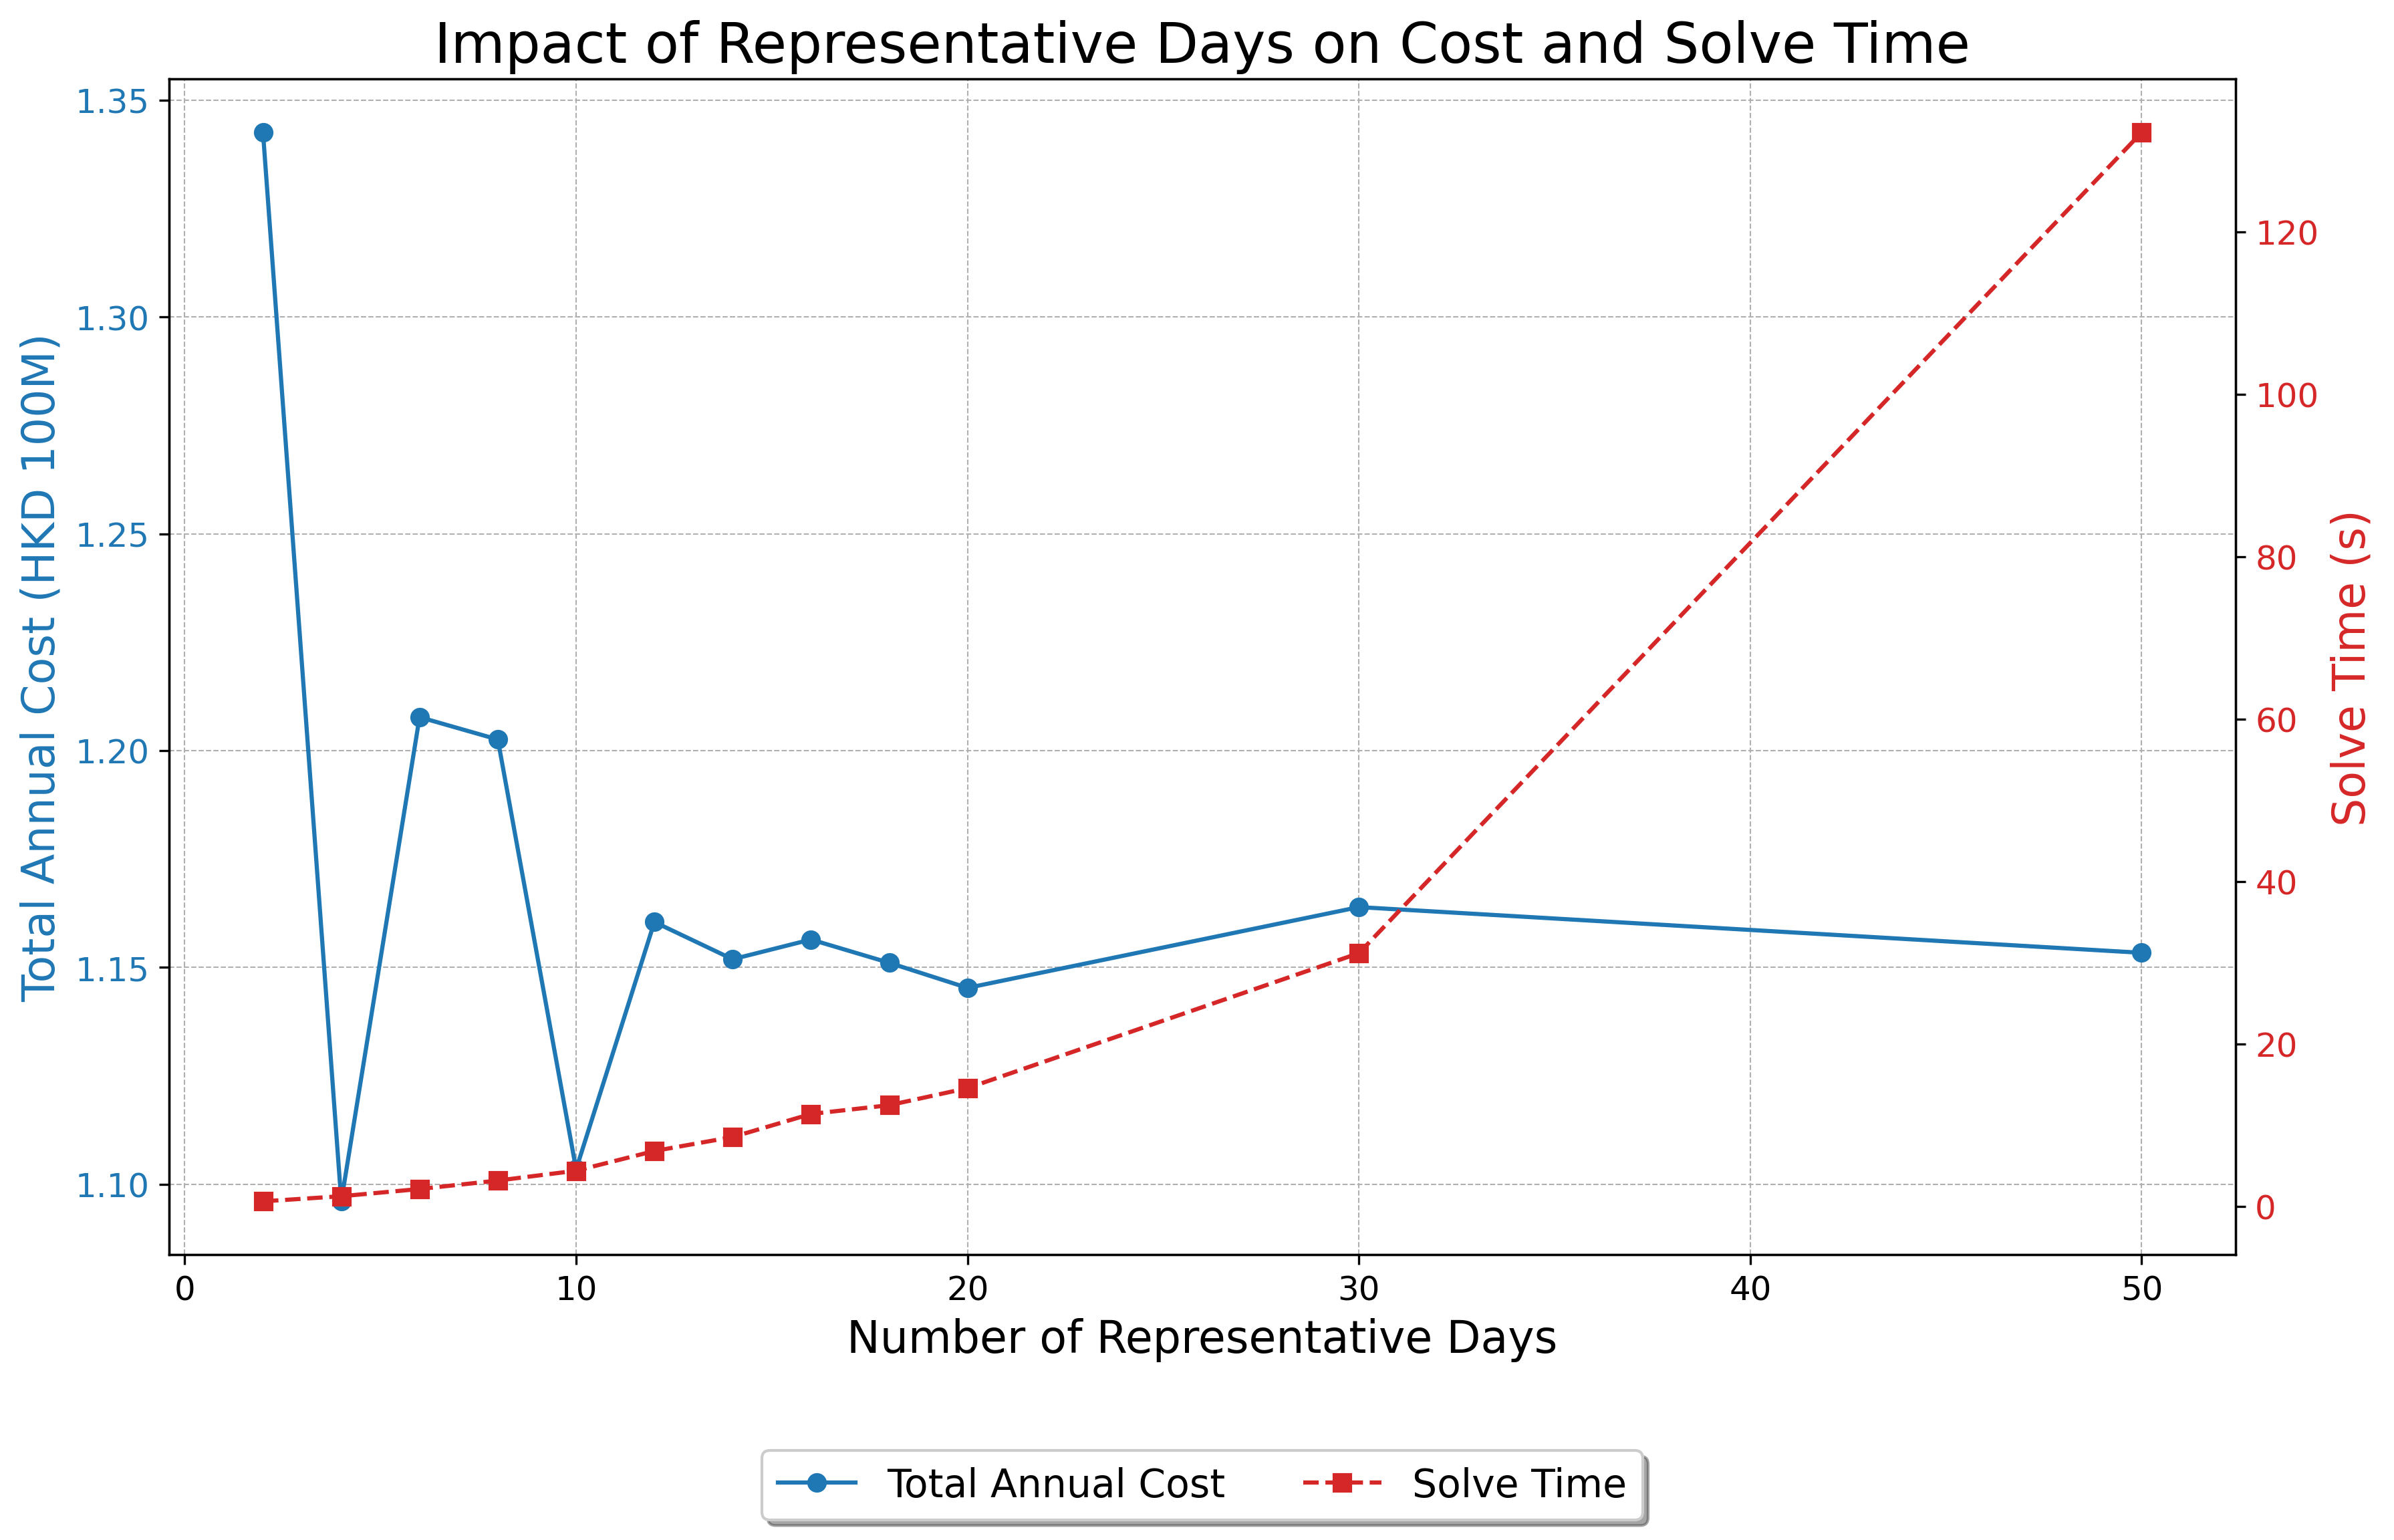
\includegraphics[width=0.9\textwidth]{plots/days_sweep_analysis.png}
    \caption{Trend of Total Annual Cost and Solve Time with Number of Typical Days}
    \label{fig:days_sweep}
\end{figure}

\subsubsection*{Analysis}
The chart above (Figure \ref{fig:days_sweep}) clearly shows the trade-off between model accuracy and computational cost:
\begin{itemize}
	\item \textbf{Computation Time (Red Line):} The solve time increases almost linearly with the number of typical days. More typical days mean more variables and constraints, which significantly increases the computational load. When the number of days increases from 2 to 50, the solve time goes from less than a second to over two minutes.
	\item \textbf{Model Accuracy (Blue Line):} The total cost shows a non-linear trend. When the number of days is small (2-10), the cost curve fluctuates a lot. This suggests that the sampling is not enough to capture all extreme weather and price conditions of the year. When the number of typical days increases to 12 or more, the total cost curve starts to stabilize within a smaller range (around 115 million HKD).
\end{itemize}
\textbf{Conclusion:} Increasing the number of typical days can describe the year's operating conditions more accurately, leading to more stable and reliable planning results. However, this improvement in accuracy comes at the cost of a sharp increase in computation time. For this project, choosing \textbf{12 to 16 days} seems to be the best balance between result stability and acceptable computation time.

\subsection{Question 3: Explanation of Weighted Operation Cost}
In this project, we use a small number of "typical days" (8 days) to simulate the operation for a full year. This method greatly reduces the calculation time while keeping a reasonable level of accuracy.

Each typical day (day $s$) does not just represent itself. It represents a whole group of days in the year that have similar weather and load characteristics. The weight $w_s$ is the total number of days in this group.

Therefore, to estimate the real total annual operational cost, we must multiply the operational cost of each typical day by the number of days it represents (its weight $w_s$). Then, we sum up all the weighted costs. If we do not use a weighted sum, we would only be calculating the cost for a few typical days, which would be much lower than the real annual cost and lead to wrong investment decisions.

\subsection{Question 4: Price Sensitivity Analysis}
We performed a sensitivity analysis on the price of natural gas by doubling it from the baseline.

\begin{table}[h!]
	\centering
	\caption{Natural Gas Price Sensitivity Analysis}
	\begin{tabular}{lccc}
		\toprule
		\textbf{Scenario} & \textbf{Total Annual Cost} & \textbf{Annual Investment} & \textbf{Total Gas Input} \\
		& (HKD) & (HKD) & (MWh/yr) \\
		\midrule
		Baseline & 120,256,069 & 39,036 & 0.00 \\
		Gas Price Doubled & 120,256,069 & 39,036 & 0.00 \\
		\bottomrule
	\end{tabular}
\end{table}

\subsubsection*{Analysis}
Since the baseline solution is already a fully electric system, further increasing the price of natural gas has no effect on the system's investment decisions or total cost. The model has already determined that even at the original price, using natural gas technology is not as economical as the "grid + storage + heat pump" combination.

\textbf{Conclusion:} Under the current parameters, the system is not sensitive to an \textit{increase} in the price of natural gas. To see gas technology being used, a sensitivity analysis with a \textit{decrease} in gas price is needed.

\section{Free Exploration and Theoretical Explanation}

\subsection{Question 5: Free Exploration - Finding the Economic Boundary for Gas Systems}

In our first analysis, we noticed that the system always chose an "all-electric" solution, with zero gas input. This led to a key question: under what economic conditions does natural gas technology (like CHP, ICE) become a valuable investment? To answer this, we conducted a two-dimensional parameter sweep, systematically exploring the impact of both \textbf{natural gas price} and \textbf{gas equipment investment cost} on the optimal system design.

\subsubsection*{Experiment Design}
We simultaneously reduced the natural gas price (from 100\% to 10\% of baseline) and the investment cost of all gas equipment (CHP, ICE, Gas Boiler) (from 100\% to 10\%) and observed if the system's strategy would fundamentally change.

\subsubsection*{Findings: The "Phase Transition" of the System's Decision}
Through batch simulations of dozens of scenarios, we successfully captured the economic "phase transition" of the system from "all-electric" to "gas-based". The heatmap below (Figure \ref{fig:gas_heatmap}) visually demonstrates this process.

\begin{figure}[ht]
    \centering
    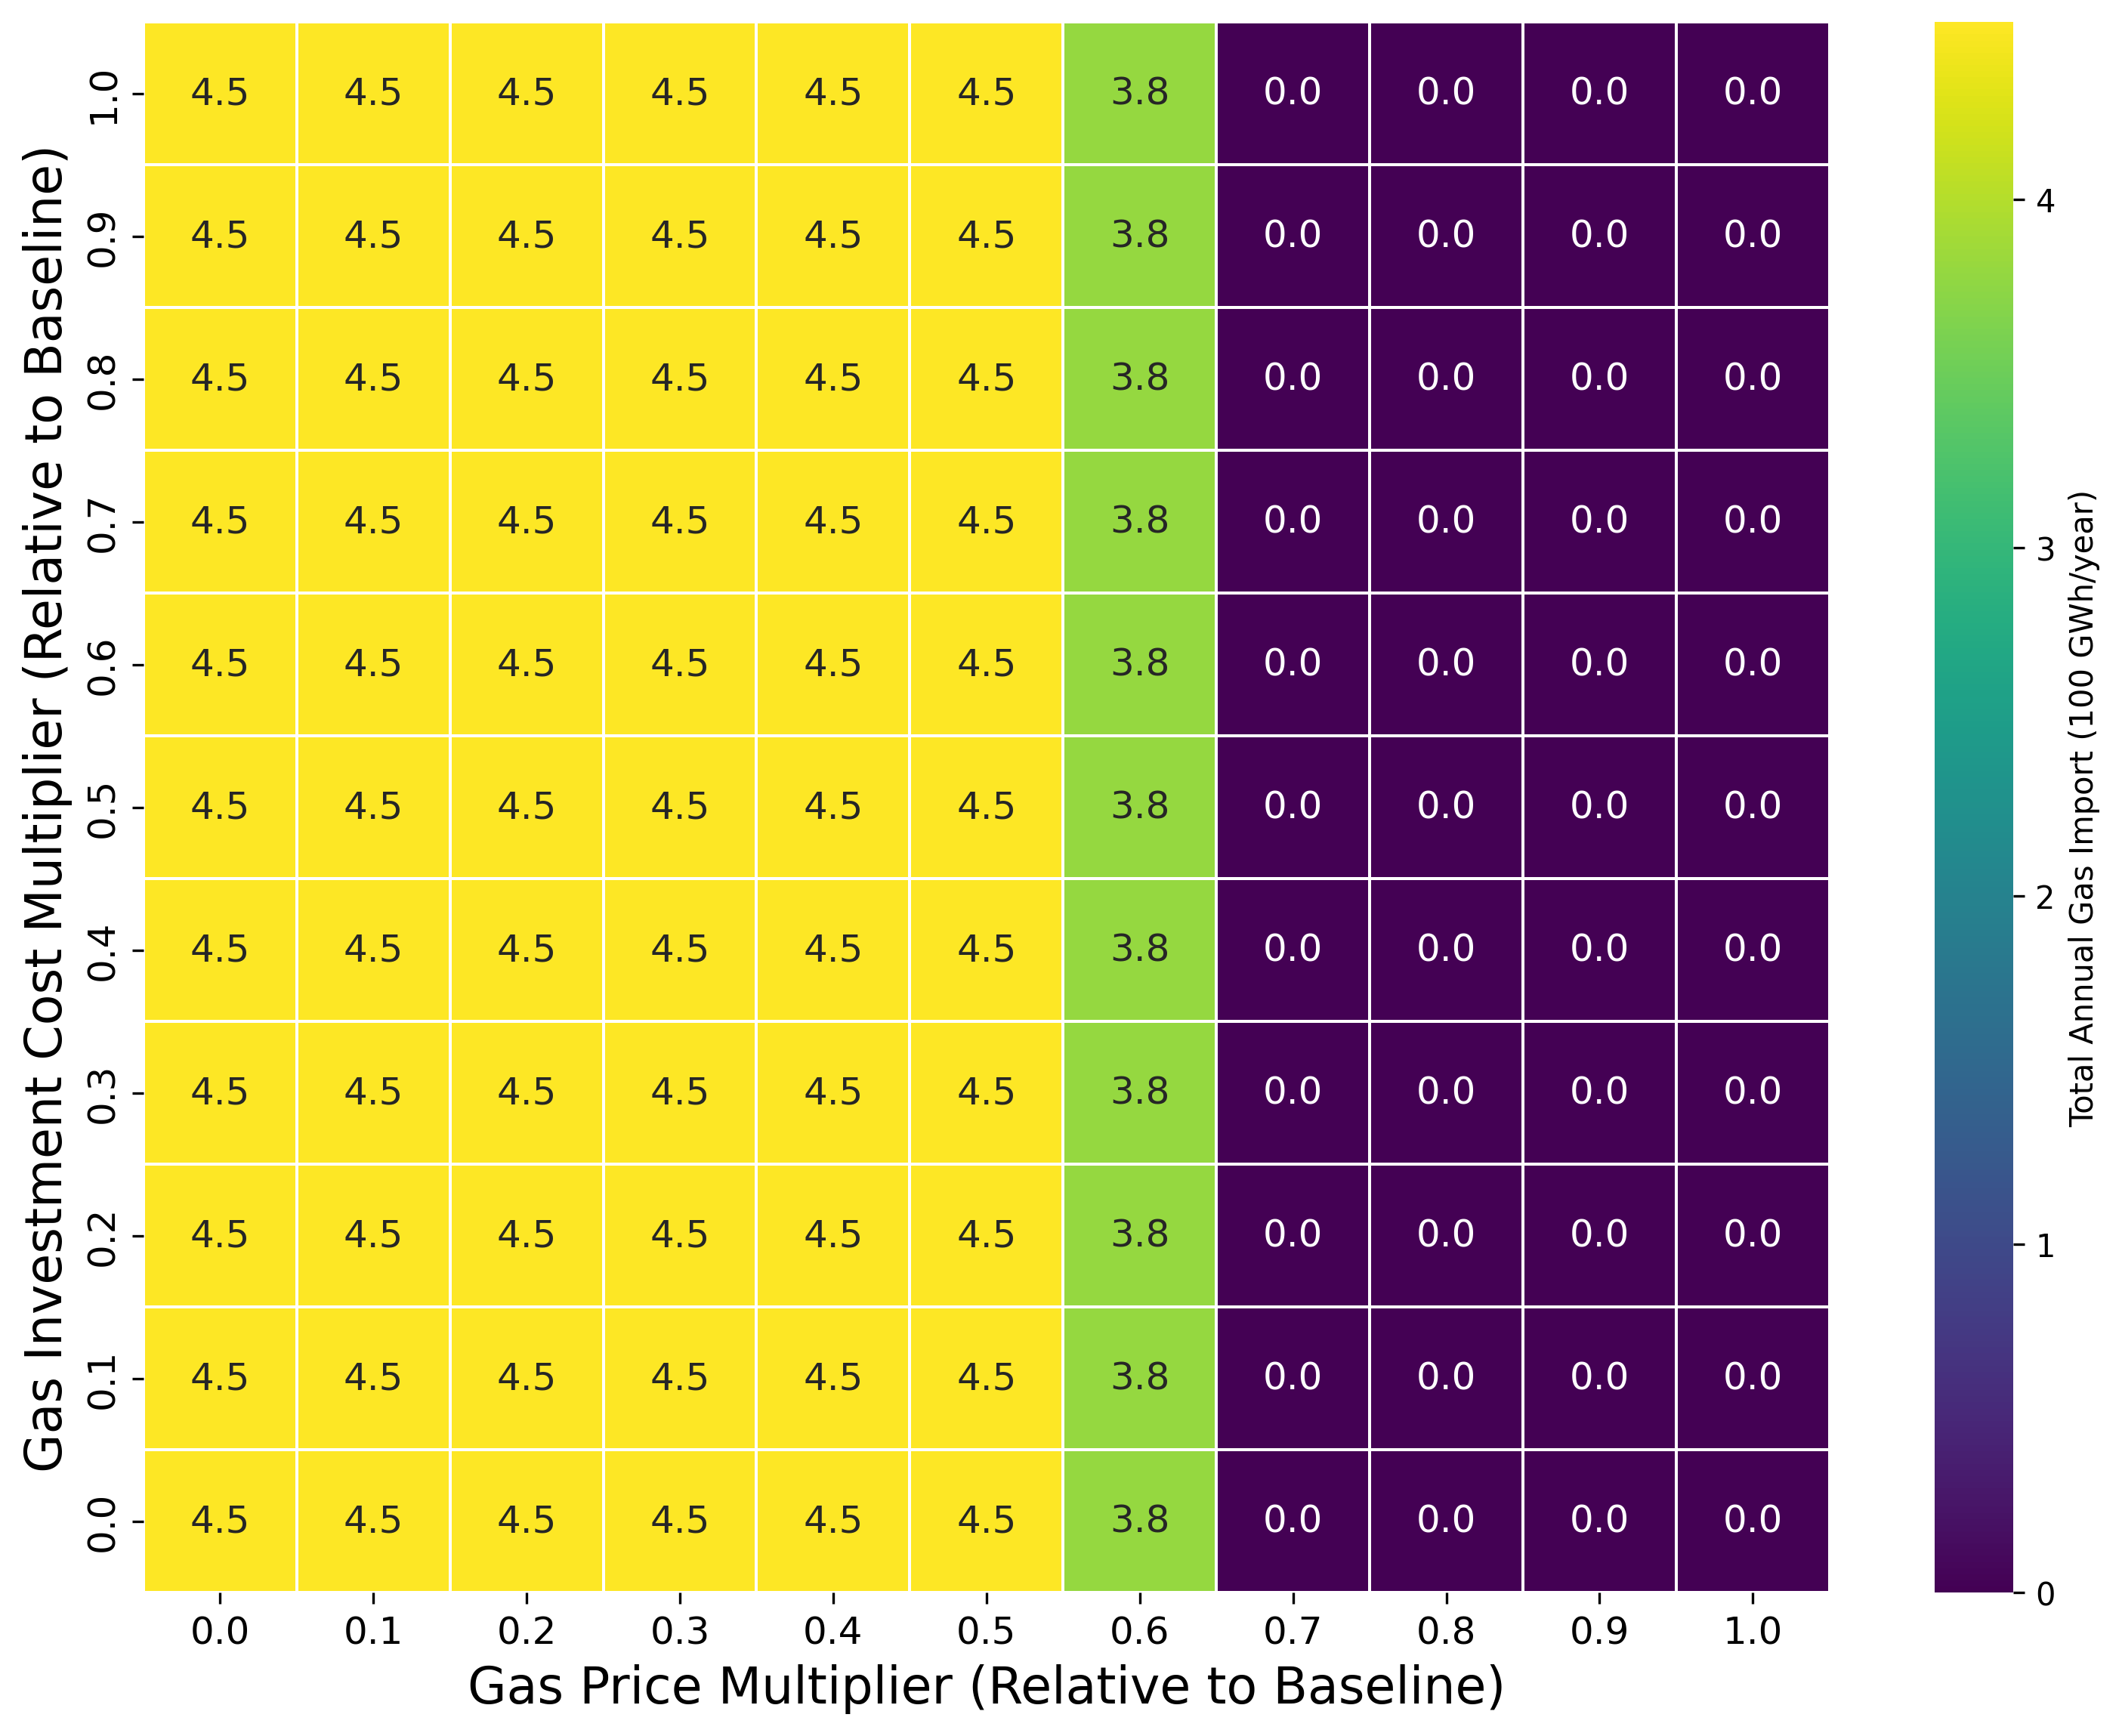
\includegraphics[width=\textwidth]{plots/gas_viability_heatmap.png}
    \caption{2D Heatmap of Total Gas Input vs. Gas Price and Investment Cost}
    \label{fig:gas_heatmap}
\end{figure}

\subsubsection*{Analysis and Interpretation}
\begin{itemize}
    \item \textbf{Identifying the Tipping Point:} From the data, we can clearly see that when the gas equipment investment cost is held constant, the natural gas price needs to drop to \textbf{60\%} of the baseline price for the system to make a fundamental change. At this point, the total cost begins to drop significantly, and the system starts to invest heavily in ICE (136 MW), formally introducing natural gas into the energy mix.
    \item \textbf{The Victory of Economic Trade-offs:} Once this tipping point is crossed, the economic advantage of natural gas becomes clear. For example, when the gas price is at 50\% of baseline, even with 100\% investment cost for gas equipment, the system's total cost drops from 120 million to 104 million HKD. In this case, the model chooses to use a large amount of natural gas (450,000 MWh/year) to power ICE for combined heat and power generation, which is more economical than relying solely on the grid and heat pumps.
    \item \textbf{ICE as the First Choice:} In all scenarios where gas investment occurred, the Internal Combustion Engine (ICE) was the preferred gas technology due to its relatively high electricity generation efficiency (35\%). This indicates that the model prioritizes maximizing electricity generation to offset the cost of purchasing electricity from the grid.
\end{itemize}

\subsubsection*{Final Finding: Redefining the Core Economic Driver}
Our initial conclusion—the "overwhelming advantage of the electricity arbitrage strategy"—now needs to be revised and deepened. Through more systematic analysis, we have reached a more precise conclusion:

\textbf{The "all-electric + storage" arbitrage strategy is indeed optimal under baseline parameters, but it is not unchallengeable. The advantage of this strategy is highly dependent on the relative price of natural gas to electricity. When the price of natural gas falls below a certain ratio to the price of electricity (around 60\% in this model), the overall energy efficiency of combined heat and power (represented by ICE) will surpass simple electricity arbitrage, becoming the new cost-optimal strategy.}

This finding provides valuable insight for energy system planners: investment decisions are not fixed, but are a dynamic balance that is highly sensitive to price signals in the energy market.

\subsection{Question 7: Explanation of the Big-M Method}
The Big-M method is a common technique in mixed-integer linear programming to convert logical constraints into standard linear constraints.

\begin{enumerate}
	\item \textbf{The Original Problem:} A storage device cannot charge and discharge at the same time. This can be written as a non-linear, bilinear constraint: $P_{charge} \times P_{discharge} = 0$. Linear programming solvers cannot handle this constraint.
	\item \textbf{Introduce a Binary Variable:} We introduce a binary "switch" variable $b$, which can only be 0 or 1. We can define $b=1$ to mean charging, and $b=0$ to mean discharging.
	\item \textbf{Linearize the Constraints:} We replace the original non-linear constraint with the following two linear constraints:
	\begin{align*}
		P_{charge} & \leq M \times b \\
		P_{discharge} & \leq M \times (1 - b)
	\end{align*} 
	where $M$ is a sufficiently large positive number.
	\item \textbf{Logical Verification:}
	\begin{itemize}
		\item When the model decides to charge, it sets $b=1$. The second constraint then becomes $P_{discharge} \leq 0$, which forces the discharge power to be 0.
		\item When the model decides to discharge, it sets $b=0$. The first constraint then becomes $P_{charge} \leq 0$, which forces the charge power to be 0.
	\end{itemize}
	In this way, we have successfully implemented an "either-or" logic using linear constraints.
	\item \textbf{Choosing the value of M:} $M$ must be greater than or equal to any possible physical upper limit of the variables involved. An $M$ that is too small will incorrectly limit the device's output, while an $M$ that is too large can cause numerical instability. In this project, the ideal value for $M$ is the \textbf{rated power capacity} of the storage device.
\end{enumerate}

\section{Conclusion}
This project successfully built an MES analysis model. Through simulation and analysis of a series of scenarios, we have drawn the following core conclusions:
\begin{itemize}
	\item In the current market environment, an all-electric solution that relies on the grid combined with large-scale energy storage is the most cost-effective option.
	\item The system's investment decisions are highly sensitive to the penalty cost for load shedding, which is a key economic lever for ensuring supply reliability.
	\item The choice of typical days (both number and quality) has a significant impact on the model's accuracy and computational efficiency, requiring a trade-off between the two.
	\item Only when the price of natural gas drops significantly relative to the price of electricity can gas technologies (like CHP) potentially enter the optimal energy system configuration.
\end{itemize}

\end{document}
